\chapter{Team 2 Agent Design}\label{team_2_agent_design}

\SetKwComment{Comment}{$\triangleright$\ }{}

\section{Core Idea and Overall Strategy}
The objective of this agent design was to implement a form of reinforcement learning to allow for an increase in performance and thus utility over time. This must be met without compromising on the overall goal of the simulations, whereby the agent must attempt to strike a balance between prioritising the micro-level goal of maximal individual utility or prioritising the macro-level goal of maximising collective utility through sustainable resource management, the latter involving a level of cooperation with the other agent types. Certain parallels can be drawn to evolutionary ecology, as the Tower with the Resident agents can represent a closed ecosystem, with the Platform providing a limited food source.
\subsection{Teleo-Reactivity}
Residents of the Tower are simulated as autonomous agents, which are functioning within an uncertain environment. Each agent has the individual goal of survival, and each agent is able to sense the amount of food on the Platform, upon its arrival at their floor. Thus, the immediate actions of the agents are to achieve the goal of survival. This can be regarded as a Teleo-Reactive program \cite{NilssonN1994TPfA}, which is defined as “one whose actions are all directed towards achieving goals in a way appropriate to the current perceived state of the environment”. This sets one of the foundational design principles required for a successful agent – that is, to continuously monitor relevant information as the circumstances of the agent change. Ideally, the agent will be able to quickly adapt and be able to conduct drastic behavioural changes when required, but this can only be achieved after a certain period of learning from the environment. 
\subsection{Competitive Exclusion Principle}
Competing and cooperating with the other agents may seem to contradict the Competitive Exclusion Principle. The Competitive Exclusion Principle states that two or more species competing for the same limited resource will not be able to exist at constant populations and will inevitably lead to either the weaker competitor’s extinction, or a distinct change in its behaviour (i.e. “complete competitors cannot coexist” \cite{HardinGarrett1960TCEP}). The superior competitor generally will have an aggressive competitive advantage which leads to this. This principle aligns with our context, as our agents must satisfy their hunger with limited food being delivered on the Platform, while other team agents will do the same. Conversely, we must not cause the deaths of other agents by taking too much food for ourselves since all agents must also strive to achieve the highest collective utility possible. In order to balance these objectives, we have implemented functions unique to our agents to ensure the survival of our agent without leading to the demise of others.  

\subsection{Dynamic Adaptation}
Our goal is to create a unique advantage by allowing for the agent to experiment with different actions to different situations, until the most appropriate actions can be dynamically chosen for the future. A reward system is utilised, whereby a suitable action will be rewarded, and a detrimental action will be penalised. Given enough iterations, the agent should be sufficiently trained to consistently choose the most correct actions. This is achievable as most other agents have fixed behaviours which can be predicted by our agent; however, we also experiment with random agents to understand and quantify the change in performance and utility. Relying on a stochastic method to execute learning can result in vastly different outcomes, but it is expected that in general the agents will perform better with time.
\subsection{In the pursuit of organisation}
Under ideal circumstances, the agents will unite into an organisation where they can collectively decide the resource division strategy for that iteration. This would also allow for a pseudo-democratic justice system, whereby the agents can vote upon the reward or punishment of each other, if one respects or violates the values of the organisation. More generally, organisations can be defined as “collectivities oriented to the pursuit of relatively specific goals and exhibiting relatively highly formalized social structures” \cite{WhettenDavidA1983ORNa}. At first, there may seem to be a straightforward solution in forming an organisation, given the benefits mentioned, but formation of such a society requires great risk on the part of the agent. There are significant constraints preventing this strategy from being conveniently utilised; trust is risky and difficult to build amongst agents given the strong random nature of the environment, the food resources are too limiting to allow for the privilege of altruistic risk-taking, and the number of actions able to be taken per day are also highly limiting. These factors will result in agents somewhat selfishly prioritising survival over anything else, thus complete self-organisation will be a difficult, if not impossible to achieve within this environment. A mechanic available to agents is the “treaty”, which are formal agreements upheld by the participating agents to dictate behaviours for a set period of time. For a non-dynamic agent, this is beneficial, as it can use the knowledge of other agents to switch to a superior set of behaviours. For a dynamic agent such as ours, treaties will override any and all learning developed up to that point in the simulation and will prevent any significant learning for the duration of the treaty. Thus, it is in the best interests of a learning agent such as ours to reject all treaties, which unfortunately comes at a cost of preventing any progress to Tower-wide agent organisation. 
\subsection{Utility Considerations and Pareto Optimality}
It is not possible to maximise both individual and collective utility simultaneously. Maximising only individual utility would result in taking more resources than required to satisfy an agent’s needs to ensure that it can survive on floors with less food. This action is contradictory to maximising collective utility as it would unnecessarily reduce the resource pool for the other agents. As a result, collective utility is prioritised to enhance the survival rates of all the agents in the Tower. In principle, the consistent maximisation of the collective utility will lead to a Pareto optimal outcome, whereby there will be “no other outcome that makes one player better off without making another player worse off”. In actuality, due to the Competitive Exclusion Principle, the agents can only achieve this if they all converge their behaviours to form a single new agent type. This is the only method to ensure the collective survival of all the agents whilst also removing the competition which prevents them from maximising the collective utility (and thus achieving the Pareto optimal scenario). 
\subsection{Education and Reincarnation}
The knowledge gained over time is stored in the agent’s memory. In order to provide a more realistic simulation of the Tower scenario, each individual agent’s memory will be erased upon death. This presents a limit to the effectiveness of the learning method, as the agent’s learning rate cannot be so high that it only takes higher risk choices to learn faster, it must consider its survival. However, a separate setting was made where “reincarnation” was implemented. In this setting, upon the agent’s death, it is respawned with all the knowledge it had gained in previous lives. We use this as a comparison metric to qualitatively assess any difference in overall utility and test the model with maximum iterations to learn as opposed to just its lifespan.
\section{Strategies and Algorithms}
\subsection{Q-Learning}
Instead of using a deterministic method, we apply Q-Learning to dynamically learn a strategy for our agent based on the environment given by the game settings. The Q-Learning method we use is an extension of the classic Temporal-Difference (TD) learning.
\subsubsection{One-Step Temporal-Difference Learning}
Temporal-Difference (TD) Learning combines the attributes of Monte Carlo methods and Dynamic Programming. Like Monte Carlo, TD has the ability of online learning from the specific feedback that the agent receives without the need to construct a model of the environment. In addition, TD is equipped with the advantage of Dynamic Programming. It is able to update the estimates of the current state based on other estimations of future states, which means that it is not necessary for TD learning to wait for the final outcome when updating the strategies \cite{alma991000179099701591}.
\begin{equation}
    V(S_t) \leftarrow V(S_t)+\alpha[R_{t+1} + \gamma V(S_{t+1}) - V(S_t)]
\end{equation}
where $V$ is the value of states and $R$ is the reward for transferring to some state.

The $R_{t+1} + \gamma V(S_{t+1})$ term is the reward for transferring to the next state plus the time-decayed value of the next states. This is the approximation of the Markov Reward Process if we keep iterating this step until reaching the final state. Thus, $R_{t+1} + \gamma V(S_{t+1})$ can be considered as a better estimation of the value for the current state. In this case, it can be easily observed that $R_{t+1} + \gamma V(S_{t+1}) - V(S_t)$ is the error between our estimated current state value and its better approximation. Finally, the value of the current state is re-estimated with this error plus its previous estimated value.  

The TD learning method has been proven to be able to converge. It is not difficult to imagine that if we maintain this updating process for the values of all states, we will be able to reach a good approximation to the value defined in the Markov Reward Process.

\subsubsection{Q-Learning Algorithm}
Q-Learning is an off-policy version of the Temporal-Difference method.

Instead of only considering the transition between states, policies and actions are introduced in Q-Learning. An action is a behaviour that the agent can perform under some situation. A policy is the behaviour for an agent at a given time, which can be interpreted as the mapping from a given state to a given action corresponding to that state. For an off-policy algorithm, the policy that is evaluated and improved can differ from the policy that the agent will take to introduce the action. In other words, we may update our strategy under the assumption that the agent will take one action in the next state, but the agent may eventually take another action.

In Q-Learning, the transition between state-action pairs is involved. The state-action pairs also belong to the Markov Reward Process as in the TD method. Q value measures the value of a state-action pair which means that Q value tells the quality of taking one action under given state. Moreover, a Q table is a combination of all the Q values which includes all the possible states and corresponding actions along with their Q values  \cite{alma991000179099701591}. 

In terms of the actual policy of an agent in Q-Learning, we combine the exploration policy and greedy policy. In greedy methods, the agent selects an action which has the highest quality under the current state. In greedy methods, the agent selects an action which has the highest quality under the current state. In other words, the agent will select the action with the highest Q value in that state. The exploration policy introduces a probability  $\delta$, which is the probability that the agent will ignore past experience (i.e., the Q table) and explore potentially better results. In summary, the agent will have a probability of $\delta$ to take a random action and a probability of $1-\delta$ to follow the greedy policy. 

The Q table is updated with the following function
\begin{equation}
    Q(S_t, A_t) \leftarrow Q(S_t, A_t)+\alpha\left[R_{t+1} + \gamma\max_{\alpha}Q(S_{t+1},a)-Q(S_t,A_t)\right]
\end{equation}
The updating function is nearly the same as that in TD learning except that we now measure the value of a state-action pair. The error between the estimated Q value and the better estimated Q value of the current state is also utilised in the updating process. Although the agent has a probability to take the random policy, we assume that the agent acts according to the greedy policy for updating which is expressed in the term $\max_{\alpha}Q(S_{t+1},a)$. Such setting ensures a stable but exploratory learning process and that is why Q-Learning belongs to the off-policy category.

\subsection{Hill Climbing}
To improve the process of changing strategies we implement the Policy Hill-Climbing (PHC) algorithm, which is a simple extension of Q-learning. PHC is a simple adaptation that performs the hill-climbing algorithm in the space of mixed strategies.  Here, the starting point of the policy space is initialised so that all policies have a uniform probability, unlike the more common random initialisation of probabilities. The PHC algorithm is formulated in Algorithm \ref{phc-algorithm}.

\begin{algorithm}
\caption{PHC Algorithm}
\label{phc-algorithm}
$\alpha\in(0,1]$\Comment*[r]{Learning rate}
$\beta\in(0,1]$\Comment*[r]{Learning rate}
$Q(s,a)\leftarrow0$\;
$\pi(s,a)\leftarrow\frac{1}{\left|A_i\right|}$\;
\Begin(\Comment*[h]{Perform each iteration}){
	$a\gets\pi(s)$\;
	$Q(s,a)\leftarrow (1-\alpha)Q(s,a)+\alpha\left(r+\gamma\max_{\alpha}Q\left(s',a'\right)\right)$\;
	$ \pi(s,a)\leftarrow\pi(s,a)+\begin{cases}
            \beta &\textrm{if } a=\operatorname{argmax}_{a'}Q(s,a)\\
            \frac{-\beta}{|A_i|-1} &\textrm{otherwise}
            \end{cases}$\;
}
\end{algorithm}

PHC keeps the Q-values as normal Q-learning would, but additionally also retains the present mixed policy. The algorithm performs non-gradient based rational optimisation by increasing the probability of selecting the action that gave the highest Q-value according to some given learning rate $\alpha$. The algorithm improves the policy by increasing the probability for selecting action with the highest Q-value according to the learning rate $\beta\in(0,1]$. It should be noted that for a learning rate $\beta=1$ the algorithm performs homogeneously to Q-learning as with each iteration, or step, the algorithm executes the highest Q-valued action which is precisely the greedy policy as explained earlier in Q-learning.

The PHC algorithm is only able to locate an optimal policy against stationary strategy opponents and has never been proven to converge if pitted against non-stationary strategy opponents \cite{BowlingMichael2002Mlua}. As according to $Q$, that converges at some $Q'$, the mixed strategy $\pi$ is greedy and will therefore converge to the best possible policy in response to the environment the agent is placed in. 

\section{Agent Design and Implementation}
\subsection{Design of states and actions}
As the learning involves interaction with the environment, it is essential to define the state space and the action space. A state space is a set of states, represented by vectors of observations, that an agent could possibly experience throughout its life. An action space is a set of actions that an agent could possibly perform in the game. The design of the state space and action space is tailored to the task assigned, namely maximising both individual and collective utilities. 
\subsubsection{Design of state space}
Firstly, we identified what observations are needed to determine the condition of the agent and the environment which is represented by the Tower and other agents. Considering the given task, we chose to observe four variables: 
\begin{enumerate}
    \item Our agent's HP
    \item Amount of food currently on the platform
    \item The number of days in critical condition
    \item The HP of the neighbour that is on the floor below our agent
\end{enumerate}

The first three observations served to fulfil the first aim of the task, as they could effectively reflect the health condition of our agent. The last observation was used to assess the impact of the action of our agent on the neighbouring agent, which is useful for the second aim of the task. Subsequently, we found the resolution of each observation by trial and error. Having a high resolution, the agent would be able to perceive tiny changes within the environment at the cost of increased number of states, and thus slowing the learning process. Having a low resolution, the agent would not be able to adapt to changes in the environment effectively and promptly. Finally, the state space of our agent is defined by ten state intervals for agent’s HP (0 – 9, 10 – 19, …, 80 – 89, 90 – Max HP), ten state intervals for the food on platform (0 – 9, 10 – 19, …, 80 – 89, 90 – Max food), four states for Days at critical (0, 1, 2, 3), and eleven state intervals for neighbouring agent’s HP (-1, 0 – 9, …, 80 – 89, 90 – Max HP), with an additional unknown state represented by –1, as the neighbouring agent might refuse to share such information. Table below illustrates the state space definition.

\begin{table}
\label{state-table}
\centering
\caption{State space defintion}
\begin{adjustbox}{width=\columnwidth,center}
\begin{tabular}{@{}lllll@{}}
\toprule
State Number & HP          & Food on platform & Days at critical & Neighbour’s HP \\ \midrule
0            & 0 – 9       & 0 – 9            & 0                & -1             \\
1            & 0 – 9       & 0 – 9            & 0                & 0 – 9          \\
2            & 0 – 9       & 0 – 9            & 0                & 10 – 19        \\
...          &             &                  &                  &                \\
11           & 0 – 9       & 0 – 9            & 1                & -1             \\
12           & 0 – 9       & 0 – 9            & 1                & 0 – 9          \\
...          &             &                  &                  &                \\
44           & 0 – 9       & 10 – 19          & 0                & -1             \\
45           & 0 – 9       & 10 – 19          & 0                & 0 – 9          \\
...          &             &                  &                  &                \\
440          & 10 – 19     & 0 – 9            & 0                & -1             \\
441          & 10 – 19     & 0 – 9            & 0                & 0 – 9          \\
...          &             &                  &                  &                \\
4399         & 90 – Max HP & 90 – Max Food    & 3                & 90 – Max HP    \\ \bottomrule
\end{tabular}
\end{adjustbox}
\end{table}
\subsubsection{Implementation of state space}
The state space is implemented as a 4D slice, with each dimension corresponding to columns 2-4 in Table 1. The 4D slice is then iterated through with each state being assigned an incrementing number. The state number of the agent can then be checked by accessing the 4D slice with the corresponding indices.
\begin{lstlisting}
func (a *CustomAgent2) CheckState() int {
	hp := CategoriseObs(a.HP())
	currFood := CategoriseObs(int(a.CurrPlatFood())
	critDays := a.DaysAtCritical()
	nHP := CategoriseObs(a.neighbourHP)
	return a.stateSpace[hp][currFood][critDays][nHP]
}
\end{lstlisting}
\subsubsection{Design of action space}
In the game, taking food is the main interaction with the Tower, which provides feedback according to the amount of food taken. Thus, we divided the action of taking food into six distinct actions with different number of intended food intake, as shown in Table \ref{action-space}.
\begin{table}
\label{action-space}
\centering
\caption{Action space definition}
\begin{tabular}{@{}ll@{}}
\toprule
Action number & Intended food intake \\ \midrule
0             & 5                    \\
1             & 10                   \\
2             & 15                   \\
3             & 20                   \\
4             & 25                   \\
5             & 30                   \\ \bottomrule
\end{tabular}
\end{table}

We excluded the possibility of taking more than 30 food units, as eating above this level will only bring punishment to our agent according to our reward design. Note that the intended food intakes are multiple of 5, as we would like the agent to have less actions to learn, resulting in faster convergence. 
\subsubsection{Implementation of action space}
The action space is implemented as a 2D slice. It is iterated through and assigned the appropriate food intake according to Table \ref{action-space}.
\begin{lstlisting}
for i := 1; i < actionDim; i++ {
	actionSpace[i] = actionSpace[i-1] + 5
}
\end{lstlisting} 
\subsubsection{Design of reward function}
The reward function provides a way for us to set the desired behaviour of our agent. The reward function will assess the quality of a particular action under a specific state and provide feedback, either reward or punishment, to the agent. Initially, we have designed four desired behaviours. We encourage our agent to survive, not to overeat, and to save neighbour: if the neighbouring agent is in critical state, the agent will be punished. However, the last desired behaviour was only enforced by the simple communication of "Ask HP" with the agent that is one floor below. Indeed, as shown in Table \ref{cum-death}, implementing a simple communication did not improve the agent’s performance on saving other agent, i.e., the overall death count remained the same after adding the simple communication and tuned reward function accordingly. A potential reason might be that the agent cannot learn to save with such limited information. As such, in our subsequent experiments, the simple communication was not considered, and the primary focus was placed on the first two desired behaviours.

\begin{table}
\label{cum-death}
\begin{adjustbox}{width=\columnwidth,center}
\begin{tabular}{@{}llll@{}}
\toprule
                                              &                                                                                   & Without communication & \begin{tabular}[c]{@{}l@{}}With simple\\ communication\end{tabular} \\ \midrule
\multirow{2}{*}{Cumulative death in 500 days} & Homogeneous tower (14 team 2 agent)                                               & 50                    & 78                                                                  \\
                                              & \begin{tabular}[c]{@{}l@{}}Heterogeneous\\ Tower (2 agents per team)\end{tabular} & 133                   & 139                                                                 \\ \cmidrule(l){2-4} 
\end{tabular}
\end{adjustbox}
\end{table}

\subsubsection{Implementation of reward function}
The final reward is the sum of survive bonus, eating bonus, wasting bonus and saving bonus. The individual bonuses will be explained now.
\paragraph{Survive bonus}
The survive bonus is implemented with two conditions.

\begin{algorithm}[H]
\caption{Survive bonus algorithm}
\label{survivebonus-algorithm}
\eIf{Agent is in critical state} {
surviveBonus $\gets$ surviveBonus $+1$\;
}{
surviveBonus $\gets$ surviveBonus $-(3.0\times\textrm{daysAtCriticalHealth})$\;
}
\If{Agent was in critical state before action}{
surviveBonus $\gets$ surviveBonus $+(5.0\times\textrm{daysAtCriticalHealth})$\;
}
}
\end{algorithm}

The first condition encourages actions that keep the agent in a non-critical HP state. The second condition encourages actions that take the agent out of a critical HP state (if it was in one).
\paragraph{Eating bonus}
The eating bonus is implemented by checking if the agent is in a critical condition and encourage it to eat more if it is.

\begin{algorithm}[H]
\caption{Eating bonus algorithm}
\label{eatingbonus-algorithm}
\If{Agent is in critical state} {
eatingBonus $\gets$ eatingBonus $+(0.01\times\textrm{amountOfFoodTaken})$\;
}
\end{algorithm}

\paragraph{Wasting bonus}
The wasting bonus encourages the agent to only take the amount of food that is necessary to reach maximum HP. We penalise the agent if it wants to waste food and we also penalise the agent if it does waste food. The wasting bonus is implemented with two statements.

\begin{algorithm}[H]
\caption{Wasting bonus algorithm}
\label{wastingbonus-algorithm}
wastingBonus $\gets 0.2\times(\textrm{expectedHPIncreaseWithIntendedFood}-\textrm{actualHPIncrease})$ 
\end{algorithm}

\paragraph{Saving bonus}
The saving bonus encourages the agent to perform actions that result in the agent in the floor below being in a nominal state. This is implemented with the condition which checks the agent below's state.

\begin{algorithm}[H]
\caption{Saving bonus algorithm}
\label{savingbonus-algorithm}
\eIf{Agent on floor below is in critical state} {
savingBonus $\gets$ savingBonus $-3$\;
}{
savingBonus $\gets$ savingBonus $+1$\;
}
\end{algorithm}

\subsection{Simple reward function}

Based on the health decay model defined in \ref{health-modelling}, the agent reward was designed to encourage the agent to reward a health above critical and punish dropping to critical health as well as punish overeating using a reward point value for each day. The reward function with its tuned hyperparameters is as such:
\begin{itemize}
    \item Set reward to zero for each new day
    \item If HP is 80-100 (Punish)
    \begin{itemize}
        \item $\textrm{Reward} = =0.2\times\textrm{food taken that day}$
    \end{itemize}
    \item If HP is 4-79 (Reward)
    \begin{itemize}
        \item $\textrm{Reward} = 3$
    \end{itemize}
    \item If hp is critical (Punish)
    \begin{itemize}
        \item $\textrm{Reward=10}\times\textrm{Consecutive days agent has stayed at critical}$
    \end{itemize}
\end{itemize}

When tuning the hyper parameters in the reward function appropriately, the main factors for performance tuning were cumulative total tower death count, average agent life span, and number of Team 2 agent deaths. 

\begin{table}[]
\begin{adjustbox}{width=\columnwidth,center}
\begin{tabular}{@{}rrrrrrr@{}}
\toprule
\multicolumn{1}{l}{Days} & \multicolumn{1}{l}{Overeating threshold} & \multicolumn{1}{l}{Overeating} & \multicolumn{1}{l}{Critical} & \multicolumn{1}{l}{Total Death:} & \multicolumn{1}{l}{Team2 Death per agent} & \multicolumn{1}{l}{Mean Age} \\ \midrule
5000                     & 80                                       & 0.2                            & 10                           & 786                              & 8                                         & 88.14                        \\
5000                     & 80                                       & 0.2                            & 5                            & 863                              & 7                                         & 72.94                        \\
5000                     & 80                                       & 0.2                            & 1.5                          & 876                              & 10                                        & 63.44                        \\
5000                     & 80                                       & 0.2                            & 3                            & 844                              & 7                                         & 73.11                        \\
5000                     & 80                                       & 0.2                            & 15                           & 913                              & 6                                         & 71.63                        \\
5000                     & 70                                       & 0.2                            & 10                           & 797                              & 12                                        & 71.61                        \\
5000                     & 60                                       & 0.2                            & 10                           & 830                              & 13                                        & 82.71                        \\
5000                     & 80                                       & 0.5                            & 10                           & 859                              & 9                                         & 80.48                        \\
5000                     & 80                                       & 1                              & 1                            & 865                              & 6                                         & 69.33                        \\ \bottomrule
\end{tabular}
\end{adjustbox}
\end{table}
\begin{enumerate}
	\item Tuning the overeat threshold down meant fewer overall deaths, but more team2 agent deaths, a rough optimal value was found at 80 hp. Setting a higher threshold would have the opposite effect
	\item Tuning the overeat punishment parameter seemed to have little impact on agent behaviour as the agent would understand punishment regardless of severity and try to stay below the overeat threshold. An optimal value was found at 0.2*(food taken that day)
	\item For tuning the critical health status punishment parameter, if agent was punished less for having consecutively critical hp meant fewer overall deaths, but more team2 deaths. Setting a stronger punishment for this gave the opposite effect. The value for this parameter giving best performance on average was at 10*(days agent has stayed at critical consecutively)
\end{enumerate}

The values found for tuning are only estimates of what gives best agent performance in synergy with the tower. This is because the tower introduces a very strong randomness effect as it reshuffles the agent floor locations after only one day. This means almost no run will ever be the same and highly unlucky events, with for example no food for several days, are very likely to occur. 

\section{Results and analysis}
\subsection{Aim of the simulations}
The aim of these demonstrations, as outlined throughout the report, was to design and produce an agent that could display the survivability of a reinforcement learning agent. The agent was intended to attempt to strike a balance between prioritizing individual utility through survival, and collective utility through sustainable behaviour with resources. This was to be done with the principle of Teleo-Reactivity in mind, whereby the agent must take actions to pursue the goal of survival by dynamically adapting to the environment using perceived information. As such, for the demonstration to be considered successful, the final design of the agent should display how it learns through reinforcement learning, with the core strategies combined with Q-learning and Hill Climbing and the environmental response, to survive in the Tower along with other agents. This includes utilising the design of states for q-table and reward formula, as well as demonstrating taking a variety of actions before died. This in turn would culminate into a converge reinforcement learning agent. This section aims to highlight how the agent achieves each of the environments by going through the survivability of the reinforcement learning agent in the environment with different hyperparameters. 

The performance of our agent will be justified by metric relating to both individual and collective utility: reward by day, cumulative reward by day, HP vs day, and food taken per day (HP), and age lived per generation.

\subsection{The performance of our agent}
As mentioned, the performance of our agent will be measured with metrics involving reward, HP, food taken, and age. For a reinforcement learning agent, cumulative reward is often used to judge a reinforcement learning algorithm. The reward that the agent receives while acting and learning tells how well the algorithm performed while being deployed. On the other hand, the plot for HP vs days describes the survivability in the environment (Tower in this situation).
\subsubsection{Convergence}
\begin{figure}
\centering
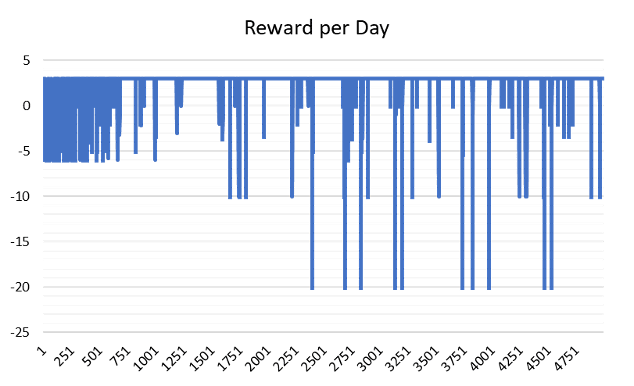
\includegraphics{004_team_2_agent_design/rewardperday}
\label{rewday-team2}
\caption{Reward per day}
\end{figure}

\begin{figure}
\centering
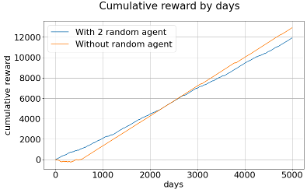
\includegraphics{004_team_2_agent_design/cumrewardbydays}
\label{cumday-team2}
\caption{Cumulative reward against days}
\end{figure}

Figure \ref{rewday-team2} is the result of a simulation for 5000 days without random agents. Reincarnation is allowed in this simulation. 

It can be observed that during approximately the first 500 days, the agent consecutively gets punished and the reward fluctuates frequently. Then, it starts to find the way to cater to the design of reward function, and despite the instability caused by randomness in the Tower, the reward function tends to be smoother, as the changes in reward function occur less frequently. 

In addition, in Figure \ref{cumday-team2}, we can find that the cumulative reward increases at a nearly steady speed after fluctuation. The turning point is approximately 500 days as well.

Thus, it can be concluded that under the configuration of this experiment, the policy of the agent is able to converge at around 500 simulation days. This means that the agent manages to find the best policy to maximise the reward he can get and persist this policy to consecutively achieve better rewards. Within its context and ability, it has achieved the Pareto optimal level for individual utility.

The verification of convergence is fundamental to the presentation of our results. All the results introduced next are based on our successful implementation of the learning algorithm.

\subsection{Random Agent}
The effect of having random agents in the Tower to our agent is discussed in the following. The random agent takes food randomly with the range between 1 till max food available on the platform. This strategy can result in the random agent overeating, which will reduce collective utility. This is due to total food allocation equal to $(\textrm{FoodPerAgentRatio}) * (\textrm{number of agent})$ while the random agent will intend to eat between 1 and total food allocation.
\begin{figure}
\centering
\label{team2av}
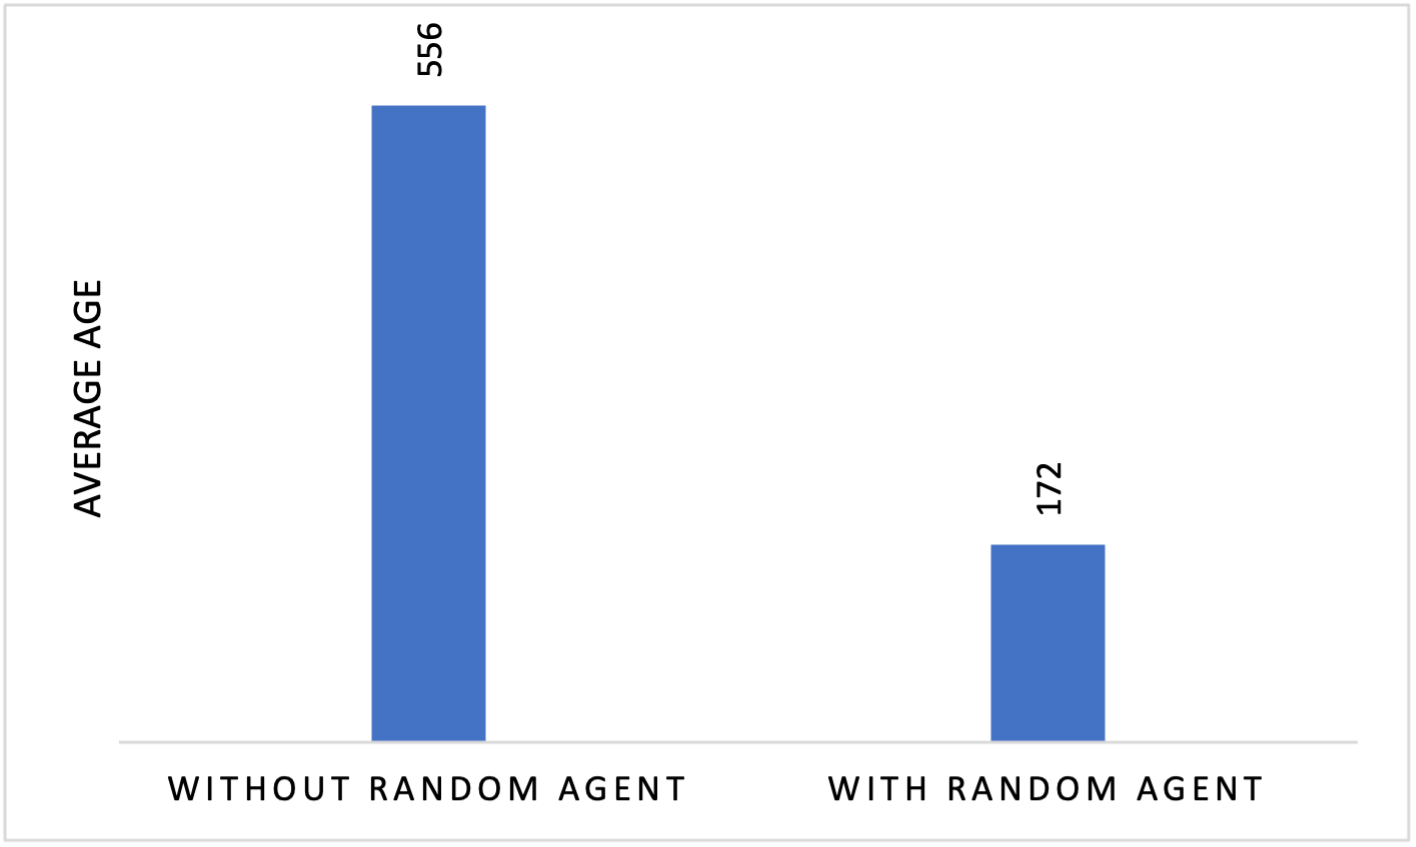
\includegraphics{004_team_2_agent_design/team2avage}
\caption{The average age of Team 2 Agent}
\end{figure}
\begin{figure}
\centering
\label{cumreward-team2}
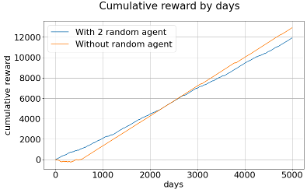
\includegraphics{004_team_2_agent_design/cumrewardbydays}
\caption{Cumulative reward by days}
\end{figure}
\begin{figure}
\centering
\label{dayreward-team2}
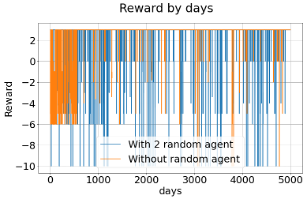
\includegraphics{004_team_2_agent_design/rewardbydays}
\caption{Reward by days}
\end{figure}
\begin{figure}
\centering
\label{hpchange-team2}
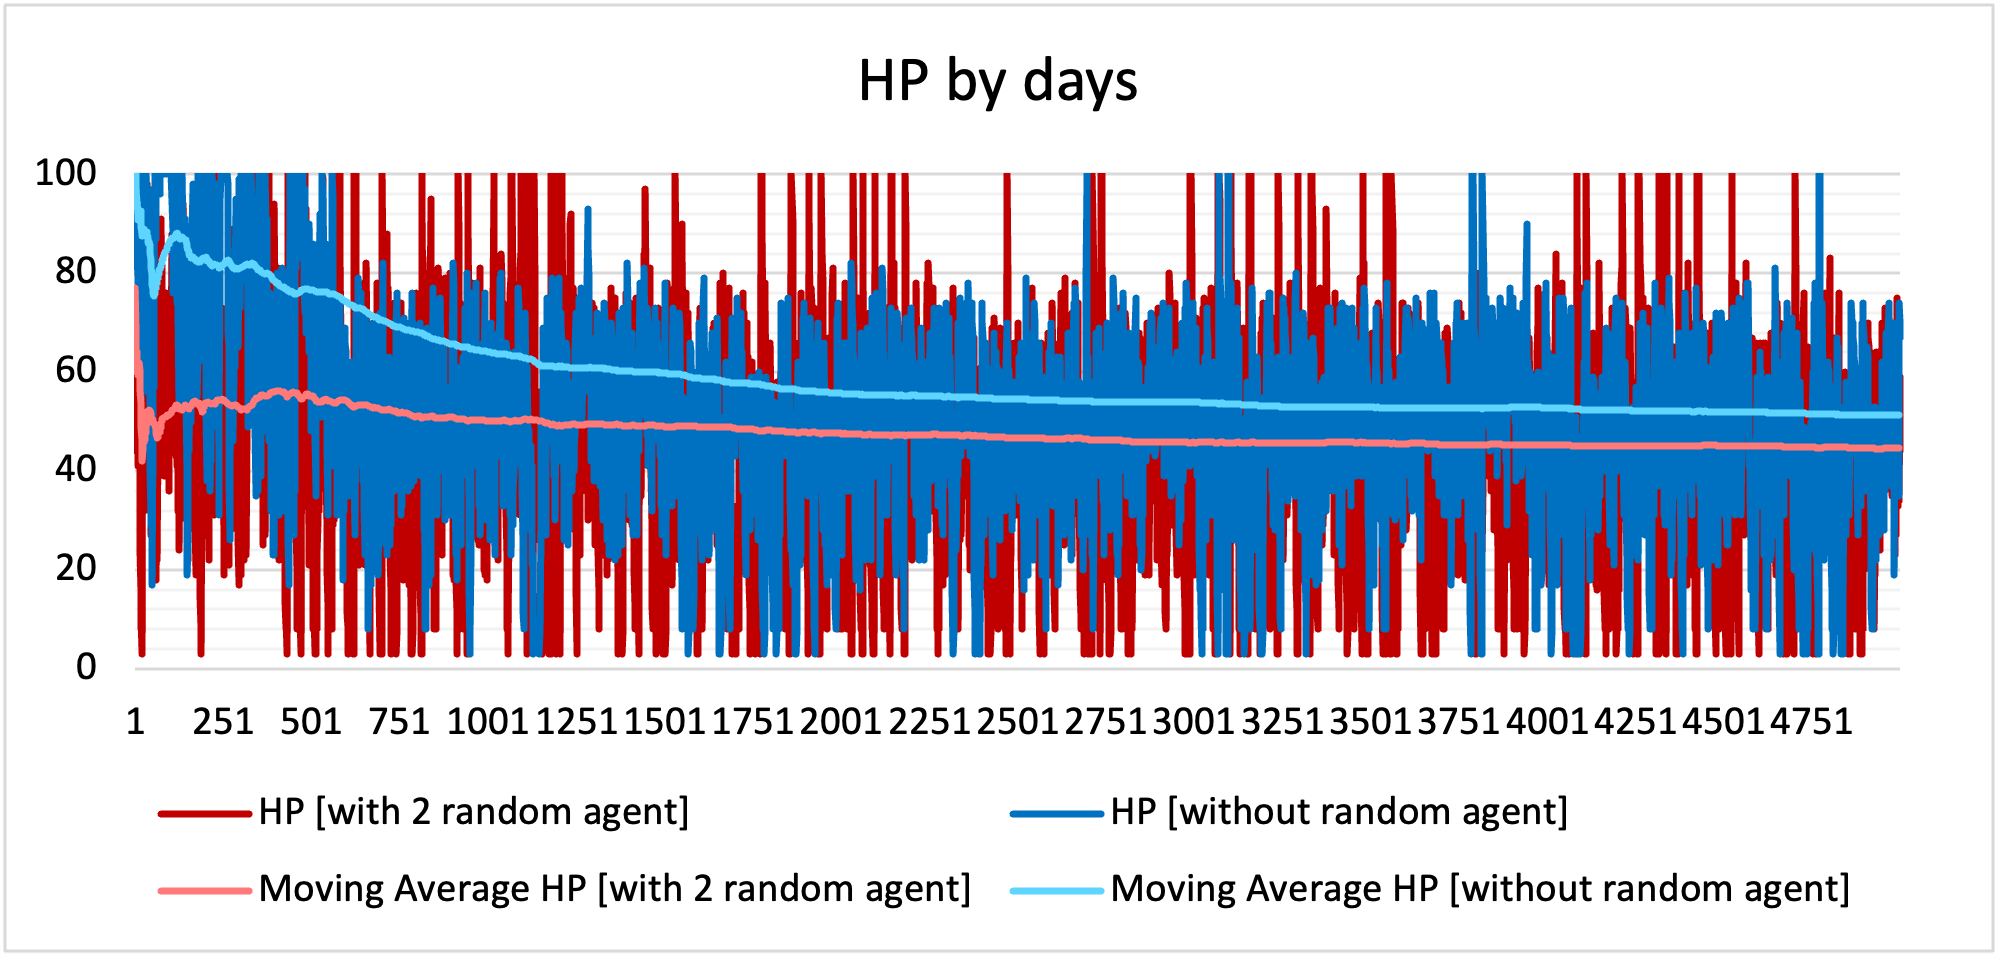
\includegraphics{004_team_2_agent_design/hpchange}
\caption{The change of agent HP by days}
\end{figure}

With the inclusion of the random agent(s) in the Tower, the average age of our agent is observably decreased from 556 days to 172 days in Figure \ref{team2avage}. This demonstrates the direct implication of collective utility on an individual agent; regardless of individual strategies, a rogue agent which does not keep the macro-level goal of collective utility will hamper the individual utilities of the other agents. 

The results in Figure \ref{cumreward-team2} and Figure \ref{dayreward-team2} are from a reincarnation-allowed simulation with only one agent of our team. In figure x.2, our agent with 2 random agents performs better than without random agent before 2500 days. However, when comparing with the plot of reward by days (figure x.3), our agent with 2 random agents has a greater total reward penalty. This is due to the randomness introduced by the random agent, causing the learning process of our agent is unsufficient. On the other hand, without implementing the random agent in the Tower, our agent able to learn after being deployed.

When there are random agents in the Tower, our agent tends to overeat more frequent to confront the effect from the random agent in Table \ref{hpchange-team2}. However, the moving average HP of our agent is lower compared to without random agent.

To conclude, the random strategy of the random agent detriments the learning process of our reinforcement learning agent. The main goal for our agent is to change its strategy according to the environment to survive, the randomness effect from random agent cause confusion for our agent as the reward may be different for the same action our agent has taken at the same state. This leads to a poor learning environment for our agent and removing random agent during the learning process of our reinforcement agent is suggested.

\subsection{Average HP}
\begin{figure}
\centering
\label{avhp-team2}
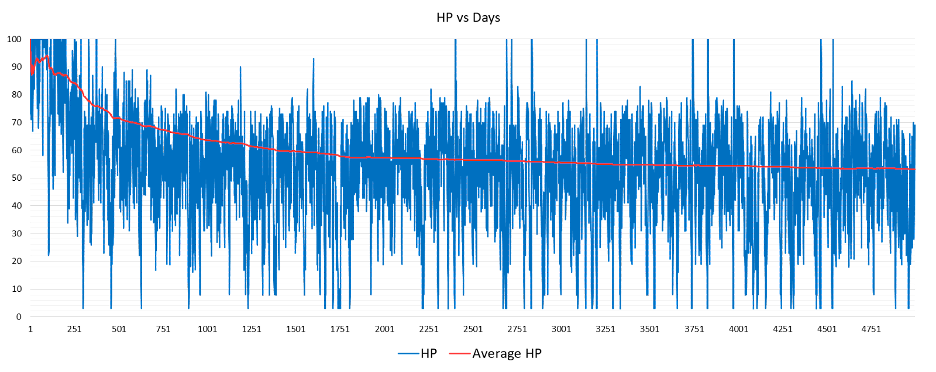
\includegraphics{004_team_2_agent_design/avhpdays}
\caption{Average HP against days}
\end{figure}

The results in Figure \ref{avhp-team2} are from an experiment without random agents. Only one agent of our team is included, and reincarnation is allowed. 

Following the design in the reward function, the HP of our agent is learnt to retain under 80. It does not choose to stay as close as possible to the upper HP limit 80. Instead, the agent decides to maintain the HP around 55 on average. 

This may indicate that staying at a high HP level may not be a good surviving strategy in the tower. 

\subsection{Reincarnation of agent}
The results of this part are from experiments without random agents and only one agent for our team is involved.

With reincarnation, the agent will not be able to lose its memory or experience after each death, which is a basic factor for a learning algorithm. In our hill-climbing Q-learning, the reincarnation allows for the retention of the Q table and policy table when the agent dies. 

From the comparison of Figure \ref{rewday-team2} and Figure \ref{cumday-team2}, it seems that there is no difference between the agent with and without reincarnation in terms of the total death and surviving days. The agent without reincarnation can live as long as the agent with reincarnation although it cannot inherit. This is partly because that, due to our effort in design to minimize the model complexity and maximize the convergence speed, our agent learns fast and normally it will converge within 200 days. Thus, if the agent can avoid death in the first 200 days, which is of high probability, it can live for a long time with the learnt strategy. Its policy will be self-optimized consistently as long as he is alive. 

This can be further explained by examining the Figure \ref{team2av} graph that specifically shows the 13th life of the non-reincarnating Team 2 agent from Figure \ref{rewday-team2} Here the agent although not reincarnated from a previous life still shows a cumulative reward curve that eventually shows a linear increase, meaning it has found a near optimal policy through dynamically adapting fast enough.

In addition, the loss of reincarnation still casts some instability. From Figure \ref{cumreward-team2}, we witness that the HP of the agent fluctuates more heavily if it cannot reincarnate. This may result from the fact that the most unstable duration for the Q-learning algorithm is the learning period. If the agent cannot reincarnate, it has to experience the learning period again every time it dies which will definitely introduce more unstable factors. 

\begin{figure}
\centering
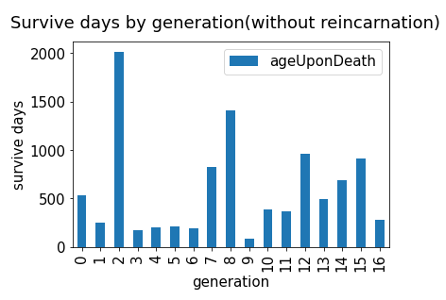
\includegraphics{004_team_2_agent_design/suvdayworein}
\caption{Surviving days of each live without reincarnation}
\end{figure}

\begin{figure}
\centering
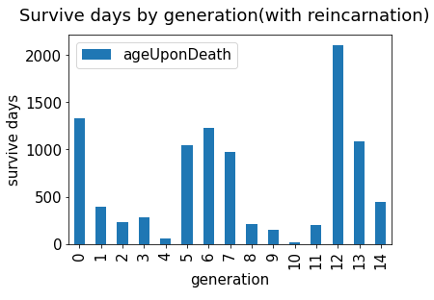
\includegraphics{004_team_2_agent_design/suvdaywrein}
\caption{Surviving days of each live with reincarnation}
\end{figure}

\begin{figure}
\centering
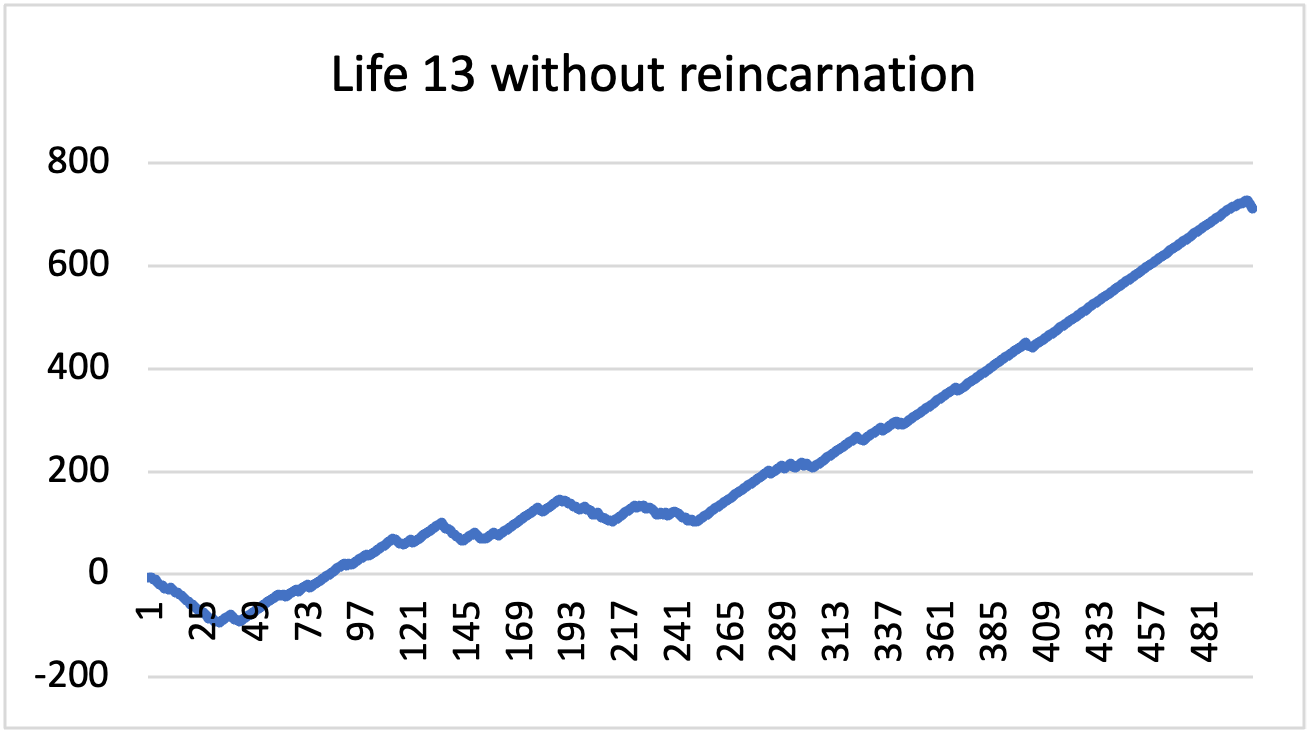
\includegraphics{004_team_2_agent_design/cum13team2}
\caption{Cumulative reward of 13th Team 2 agent life without reincarnation from the previous figure}
\end{figure}

\begin{figure}
\centering
\label{hpdaysteam2}
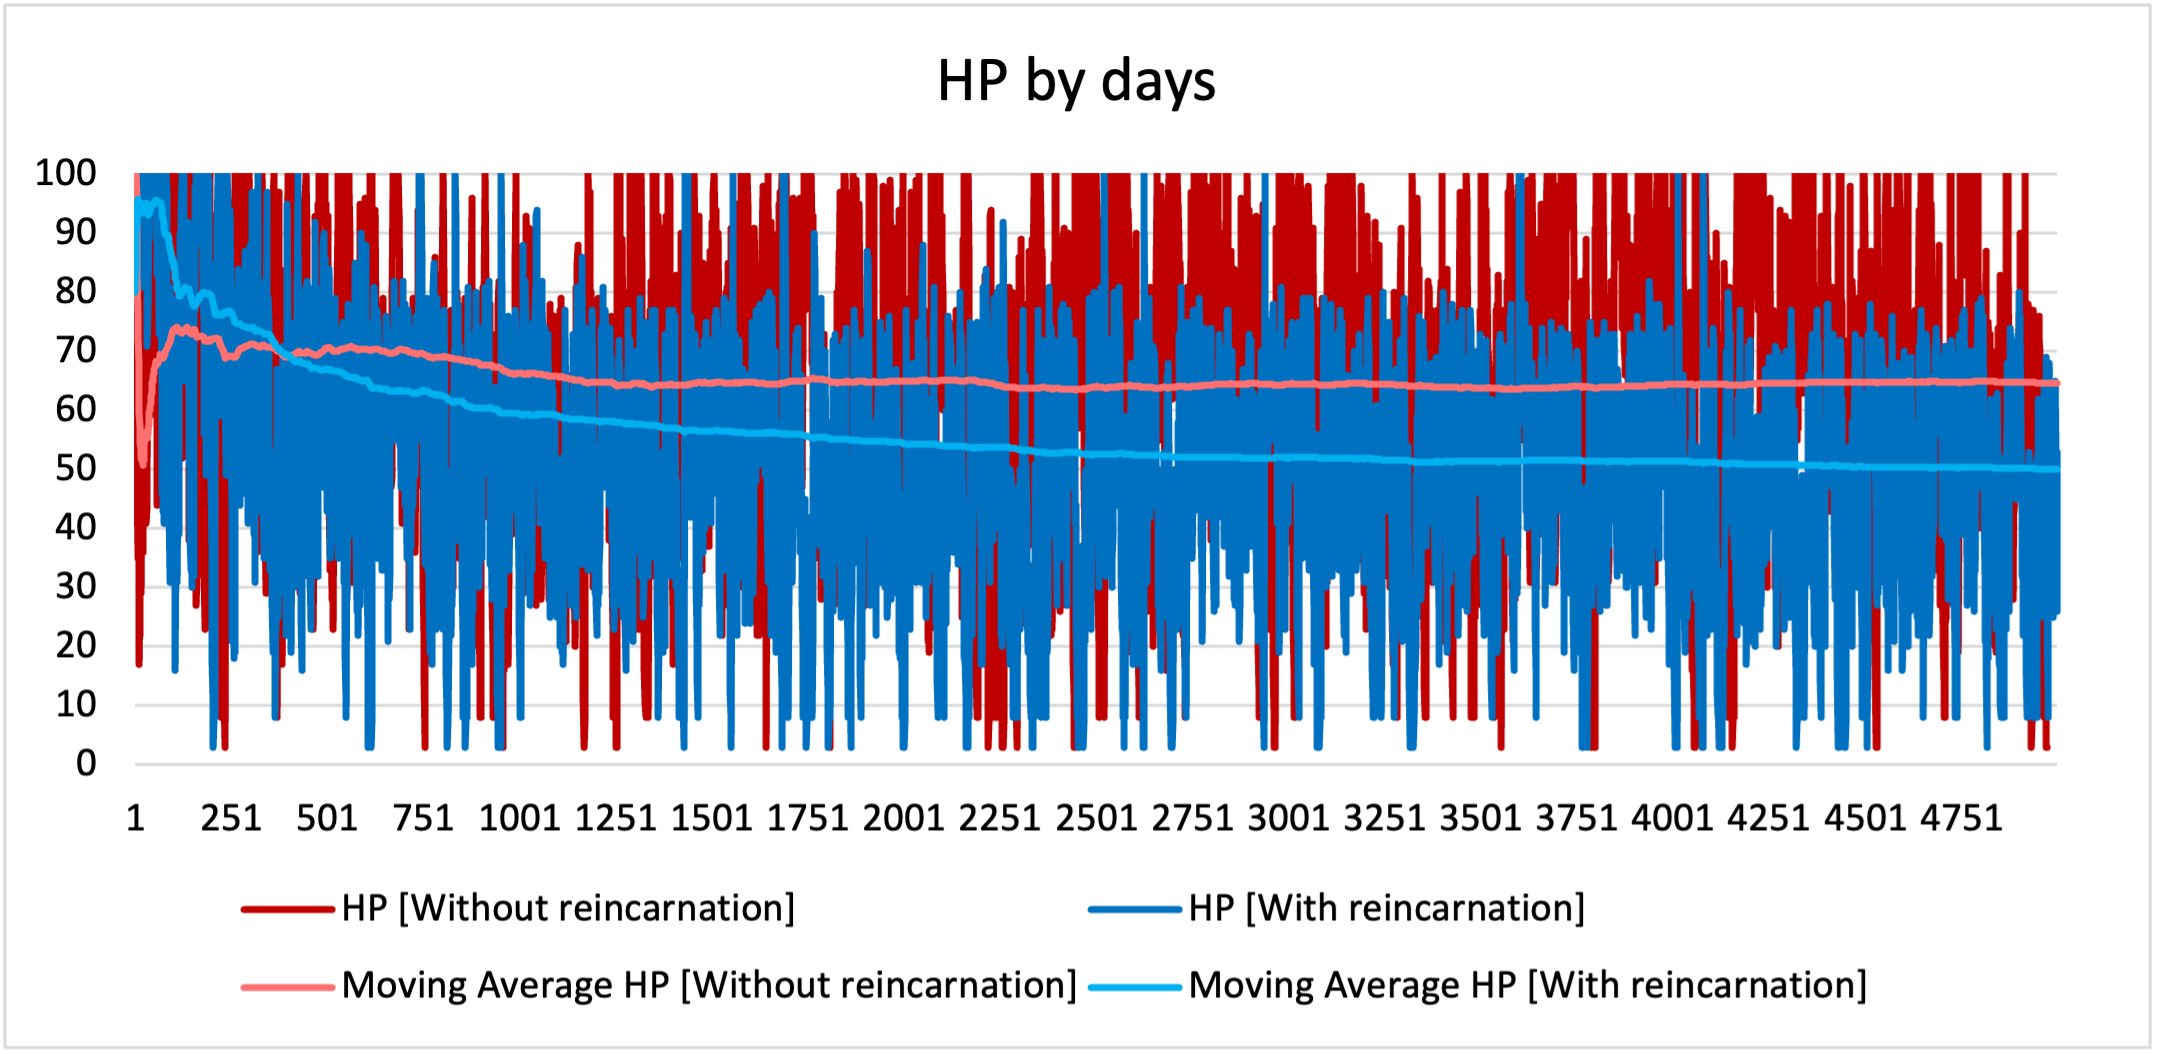
\includegraphics{004_team_2_agent_design/hpdaysteam2}
\caption{The change of HP by days with and without reincarnation}
\end{figure}

Enabling reincarnation can let the agent pass its learnt knowledge to its child, while disabling the reincarnation will lead to a tumultuous relearning process for every generation. Enabling the reincarnation of our agent is important as it let our agent learn from the reward and inherit the experience from its predecessor. 

As a conclusion to reincarnation, the most important impact of reincarnating the Team 2 agent is not an increase in its own performance as it learning rate is fast enough for the average life duration. The real trade off with reincarnation is the effect it has on the Tower’s other agents. The average HP is lower with reincarnation as can be seen in Figure \ref{hpdaysteam2}, and so the other agents benefit from this much more. As previously discussed, maintaining the Pareto optimal individual utility will allow for an increase in each other agent’s individual utilities, and thus the collective utility.

\subsection{Self-Organising Ability}
A Tower that can self-organise has reached an equilibrium where agents no longer die and instead are able to survive all together based on their adaption to each other and the environment. As discussed in SECTION A ABOUT ORGANISATION, this generally would occur when all the agent behaviours have assimilated and converged to become one and the same. Thus, it is in our interests to test a scenario with a Tower full of the same agent type. To test Team 2 agents’ own self-organising ability, Towers with different number of Team 2 agents present where tested.

The results in Figure X \ref{251team2} shows that the Team 2 agent does indeed have a huge impact on the Towers performance. The more Team 2 agents present in the Tower the fewer deaths the Tower would have. But with this reading alone its not possible to determine if the Team 2 agents actually has a self-organizing ability as there is no way of knowing when the last agent died in each run. Figure \ref{252team2} on the other hand shows how a Tower consisting only of Team 2 agents eventually reached an equilibrium point where all agents stayed alive. As such the design of the Team 2 agent showed self-organizing ability with its Q-learning PHC reinforcement learning strategy.

\begin{figure}
\centering
\label{251team2}
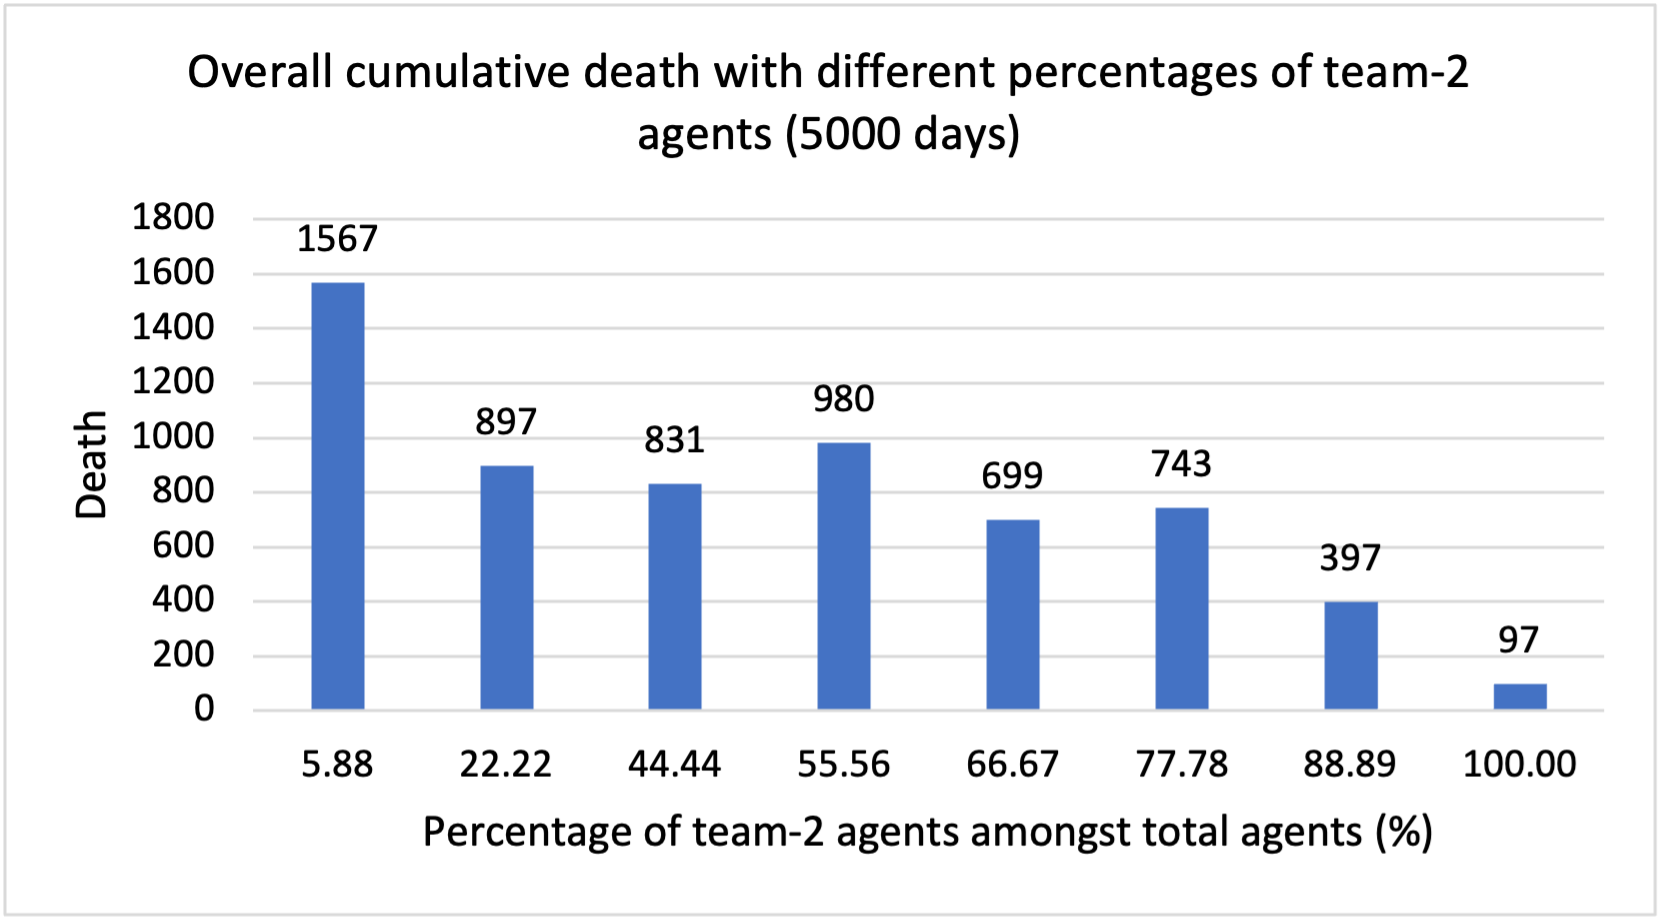
\includegraphics{004_team_2_agent_design/251team2}
\caption{1 Shows the cumulative deaths of a Towers with varying percentage of total agents being Team 2 agents. Total agent count is 18 agents.}
\end{figure}

\begin{figure}
\centering
\label{252team2}
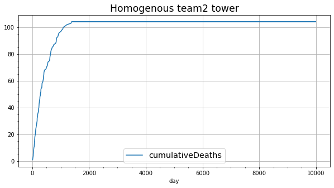
\includegraphics{004_team_2_agent_design/252team2}
\caption{Tower of only Team 2 agents reaches a point where all agents stays alive}
\end{figure}

\subsection{Learnt policies}
\begin{table}
\centering
\caption{Policy of agent when HP is 0-10}
\label{lowhp-team2}
\begin{tabular}{@{}ll@{}}
\toprule
HP   & Average Food decided to take \\ \midrule
0-10 & 27.3                         \\ \bottomrule
\end{tabular}
\end{table}
Table \ref{lowhp-team2} shows that when the HP of agent is low, the agent tends to take in as much food as he can to survive, as it must prioritise its individual survival and cannot consider other lofty altruistic goals.

\begin{table}[]
\centering
\label{midhp-team2}
\caption{Policy of agent when HP is 10-20}
\begin{tabular}{@{}lll@{}}
\toprule
HP    & Food on the Platform & Food decided to take \\ \midrule
10-20 & 0-20                 & 13.2                 \\
10-20 & 20-30                & 7.1                  \\
10-20 & 30-100               & 23.9                 \\ \bottomrule
\end{tabular}
\end{table}

From Table \ref{midhp-team2}, it is prominent that the agent is still in a dangerous HP range. When there is not much food on the platform, the agent decides to eat more to survive.
When the food on the platform is 20-30 which is still not safely sufficient, even though its HP is not high enough, the agent seems want to leave food for others. The agent probably considers that in such case, leaving food for others can be a better choice because if some agents fall into the critical level, they may need more food to reach the weak level than what they need now. Perhaps it has developed some form of empathy, where it perceives that other agents may be in similar if not more dire situations. 

When the food is abundant on the platform at this HP level, the agent takes in more food. This might be a strategy to prevent being allocated to lower floors on the next day since its HP is still near critical level.

\begin{table}[]
\centering
\label{2030-team2}
\caption{Policy of agent when HP is 20-30}
\begin{tabular}{@{}lll@{}}
\toprule
HP    & Food on the Platform & Food decided to take \\ \midrule
20-30 & 0-20                 & 16.1                 \\
20-30 & 20-40                & 6.1                  \\
20-30 & 30-50                & 21.0                 \\
20-30 & 50-100               & 5.0                  \\ \bottomrule
\end{tabular}
\end{table}

Table \ref{2030-team2} shows the decisions of the agent when HP is in 20-30 level. It is observed that its policy at this level is quite similar to that at HP 10-20. It still chooses to ensure the survival of itself when the food is not enough. When the food is above the level of scarce, it still decides to eat less and leave the food for others. In addition, when there is 30-50 food on the platform, it decides to eat more again, but when the food on the platform is more than this it chooses to barely eat. It seems that from the experience of agent in HP 20-30, 30-50 food on the platform can be a dangerous indication that it may starve or lose HP in the next few days, so he tends to supply himself for the future. And the agent considers it unnecessary to eat much when there is abundant food on the platform, due to the reward function penalties.

\begin{table}[]
\centering
\caption{Policy of agent when HP is 30-100}
\label{30100-team2}
\begin{tabular}{@{}ll@{}}
\toprule
HP     & Food decided to take \\ \midrule
30-100 & 5.0                  \\ \bottomrule
\end{tabular}
\end{table}

Table \ref{30100-team2} shows that when the HP of agent is larger than 30, it tends to eat the minimum amount of food and leave the food to others.

In summary, from the observations gathered, the learnt policy of the agent follows certain patterns:
\begin{itemize}
	\item The priority is the survival of itself; the Tower scenario is often too unpredictable to switch to more altruistic objectives
	\item Leaving food for others when the food is not sufficient tends to bring more collective benefit in the long term
	\item Maintaining HP over 30 is safer for the survival of agent and is more likely to result in a Pareto optimal value for individual utility
\end{itemize}


